\question {
    现有一个由$5$块磁盘组成的磁盘阵列,采用 RAID-5 模式,如下图所示。
}

\begin{figure}[H]
    \centering
    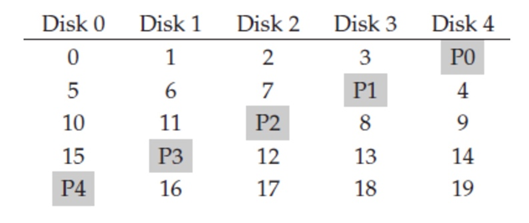
\includegraphics[width=0.6\textwidth]{img/q1.png}
\end{figure}

该磁盘阵列每个硬盘的块(block)大小为 4KB,每条(strip)含一个块;磁盘的平均寻道时间是 4ms,
旋转速度是 7200 RPM (每分钟 7200 转),传输带宽是 200MB/s,请计算:

\begin{parts}
    \part {
        平均来说,从该 RAID5 阵列上读出一个条带(stripe)的时间是多少?
    }
    \part {
        当向该 RAID5 阵列中写入连续的两个 4KB 数据块时,平均来说,所需的时间是多少?
        请考虑这两个数据块属于同一个条带和不同条带的两种情况。
    }
\end{parts}

\begin{solution}

\begin{parts}

\part

平均寻道时间为
$$
    T_{seek} = 4 \text{ms}
$$

平均旋转时间为
$$
    T_{rotation} = \frac{1}{2}(60/7200)  \approx 4.17 \text{ms}
$$

平均传输时间为
$$
    T_{transfer} = 4 \text{KB} / 200 \text{MB} = 0.02 \text{ms}
$$

因为读取一个条带,五个磁盘可以并行读取,所以总时间就是单个磁盘读取一个块的时间:
$$
    T = T_{seek} + T_{rotation} + T_{transfer} = 8.19 \text{ms}
$$

\part

写操作流程如下:

\begin{enumerate}
    \item 读旧块
    \item 读旧校验块
    \item 计算新校验块: $P_{new} = (B_{old} \oplus B_{new}) \oplus P{old}$
    \item 写新块
    \item 写新校验块
\end{enumerate}

包含 4 次磁盘访问。

对于两个数据属于同一条带的情况,两个数据块和其校验块在同一个条带,1、2 和 4、5 步可以分别同时进行。
计算时间可以忽略不计。所以共需要 2 次磁盘访问。

所需时间为:

$$
    T_1 = T \times 2 = 16.38 \text{ms}
$$

对于两个数据属于不同条带的情况,每个数据块和其校验块在同一个条带,1、2 和 4、5 步可以分别同时进行。
计算时间可以忽略不计。所以共需要 4 次磁盘访问。

所需时间为:

$$
    T_1 = T \times 4 = 32.76 \text{ms}
$$

\end{parts}

\end{solution}
